\section{Einleitung}
\subsection{Motivation}
%
%
\begin{frame}
	\frametitle{Überblick}
	\tableofcontents[currentsubsection]
\end{frame}
%
%
\begin{frame}
	\frametitle{Motivation - Kleine Katastrophen}
	\begin{figure}
		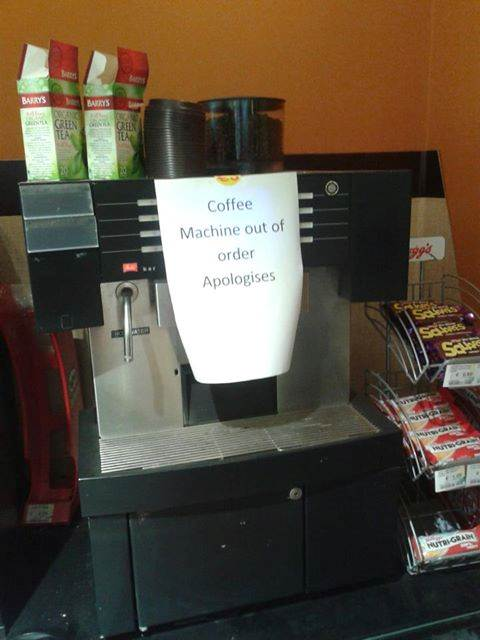
\includegraphics[scale=0.36]{grafiken/broken2}		
		\caption{Defekte Kaffeemaschine am Morgen
			\footnote{\tiny Quelle: \url{https://jlonerga.wordpress.com} }
		}		
	\end{figure}
\end{frame}
%
%
\begin{frame}
		\frametitle{Motivation - Große Katastrophen}
		\begin{figure}
			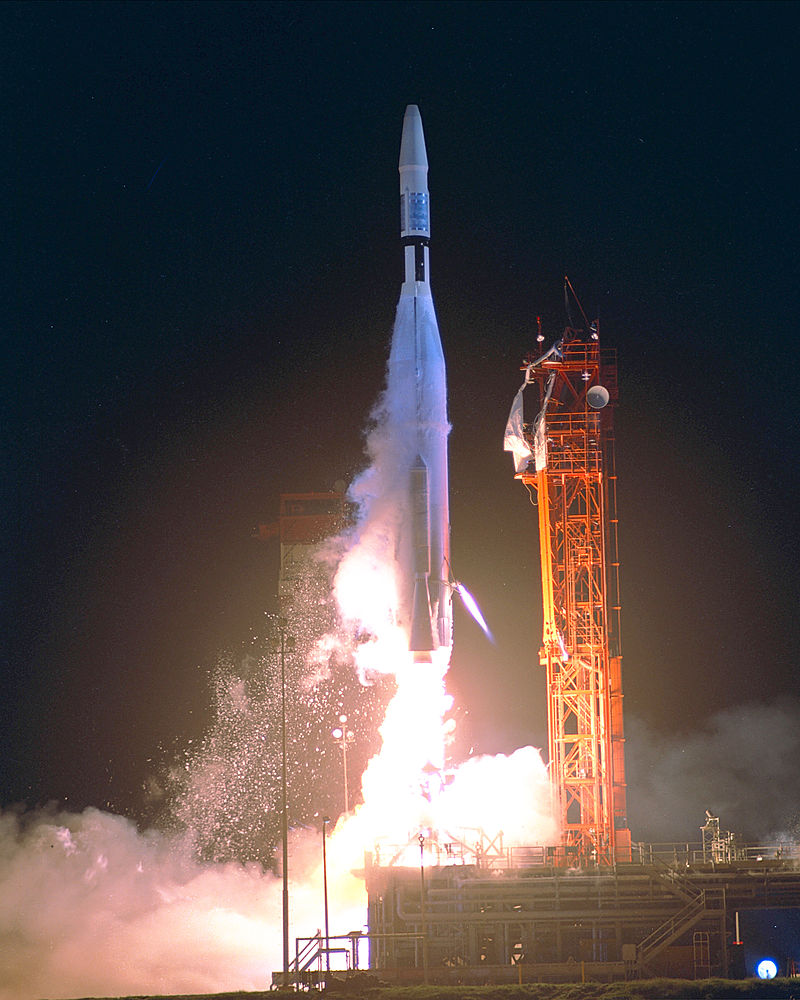
\includegraphics[scale=0.7]{grafiken/mariner}		
			\caption{Absturz der Trägerrakete der Raumsonde \emph{Mariner 1}
				\footnote{\tiny Quelle: \url{NASA} }
			}		
		\end{figure}
\end{frame}%
%
%
\begin{frame}
	\frametitle{Motivation - Lösung für kleine Katastrophen}
	\begin{figure}
		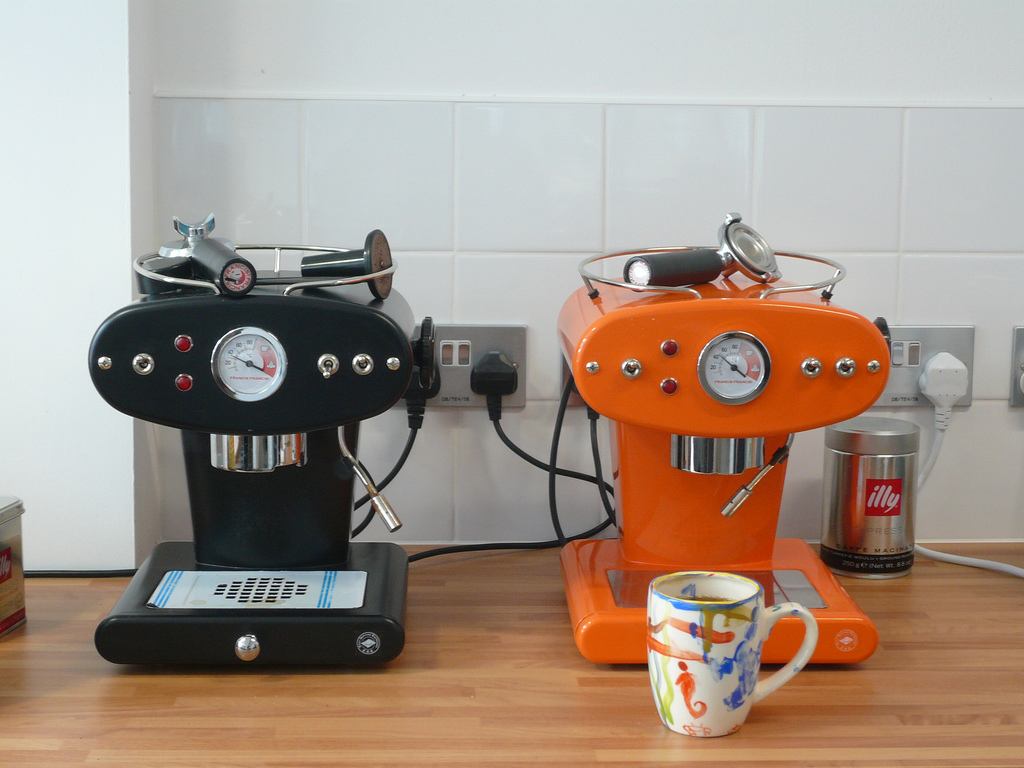
\includegraphics[scale=0.2]{grafiken/working}		
		\caption{Ansatz - Doppelt hält besser
			\footnote{\tiny Quelle: \url{http://www.sarahmei.com} }
		}		
	\end{figure}
\end{frame}
%
%

\begin{frame}
	\frametitle{Motivation - Lösung für große Katastrophen}

	
\end{frame}
%
%
%
\subsection{Ansätze für zuverlässige Systeme}
\begin{frame}
	\frametitle{Ansätze für zuverlässige Systeme - Historischer Gedanke}
	\enquote{\emph{The most certain and effectual check upon errors which arise in the process of computation,	is to cause the same computations to be made by separate and independent computers; and this	check is rendered still more decisive if they make their computations by different methods.}}
	
	- Dionysius Lardner 1834 \cite{lardner}
	
\end{frame}